%% name       : sugconf-example.tex
%% description: example of LaTeX document class sugconf
%% purpose    : illustrate use of LaTeX markup
%%              for SAS User Group conference authors
%% author     : Ronald J. Fehd for CTAN
%% date       : 8/10/2006
%% note       : all text after a percent sign (%) is a comment
%% note       : open *.pdf, <Ctrl> D to view pdf description
%% make       : pdflatex sugconf-example

\documentclass{sugconf}
\usepackage{graphicx}
%macro variables used by sugconf
\sugconfsubject{SAS 9.1.3, Microsoft Windows API, }%
\sugconfpapernumber{Paper SD01}%
%\sugconfpapernumber{\relax}%note: no paper number: warning in log
\sugconfkeywords{Base SAS, MODULEN, SASCBTBL, Microsoft Windows XP/2000, Microsoft Windows API, GetSystemPowerStatus, SAS/GRAPH}%end keywords: see in pdf description

%begin LaTeX document commands
%% NOTE: do not put newline (\\) in title nor author

\title{``Powerful''  SAS\textsuperscript{\scriptsize\textregistered} Techniques from the Windows API}
\author{Samuel T. Croker}
%\makeatletter
\usepackage[bookmarks   =false
           ,pdfauthor   ={\@author}
           ,pdfcreator  ={pdfLaTeX sugconf.cls}
           ,pdfkeywords ={\SUGconfKeywords}
           ,pdfstartview=FitBH
           ,pdfsubject  ={\SUGconfSubject}
           ,pdftitle    ={\@title}
]{hyperref}
%\makeatother
\begin{document}

\begin{abstract}Ever wonder how well that old laptop battery is performing?  Is it possible to do online tests of a laptop battery to determine the best power configuration?  Need a way to cleanly exit a SAS\textsuperscript{\scriptsize\textregistered} process when the laptop battery is low or the system switches to auxiliary power? The Microsoft Windows API provides a method for polling system power sources and SAS makes designing a simple power source querying system easy.
 Keywords: \SUGconfKeywords.
\end{abstract}

\section{Introduction}

The Windows API is a very useful group of methods and properties
that are available to developers on a Windows platform.  This type
of API is also available to many other platforms but will not be
covered by this document.  There have been several very good papers
written on how to use the Windows API so this example will only
cover the barest of details as to using the Windows API.  This application resulted from the desire to evaluate a laptop battery, and being disappointed by the cost of such applications.  So the though arose, "Why not use SAS?"  Luckily, many of the details of using the Windows API within SAS has been researched in reported in several SUGI papers.  

\section{Windows API and SAS Basics}
The functions within the Windows API must first be prototyped before
they are available to SAS.  This prototype is stored in a file
reference that has to be called \verb"SASCBTBL".  This fileref is
known to SAS and is used implicitly by the \verb"MODULEN" or other
\verb"CALL MODULEx" routines. 

For this example, the Windows API function \textit{GetSystemPowerStatus} is used to 
get information about the current power configuration.  For the \verb"GetSystemPowerStatus" function, it was necessary to experiment
a little with the informats in order to get meaningful data.  The
\verb"IB4." informat is the only informat that correctly loads the
integer data of \verb"BatteryLifetime" and
\verb"BatteryFullLifetime".  The boolean values are only correctly
loaded using \verb"IB1.".  

\begin{verbatim}
 filename SASCBTBL CATALOG 'sasuser.example.winbatt.source';
 data _null_;
  file SASCBTBL;
  input;
  put _infile_;
cards4;
ROUTINE GetSystemPowerStatus
    minarg=6
    maxarg=6
    stackpop=called
    module=kernel32
    returns=long;
* LPSYSTEM_POWER_STATUS lpSystemPowerStatus ;
arg 1 num output fdstart format=ib1.;
arg 2 num output format=ib1.;
arg 3 num output format=ib1.;
arg 4 num output format=ib1.;
arg 5 num output format=ib4.;
arg 6 num output format=ib4.;
;;;;
run;
\end{verbatim}

The SASCBTBL file begins after the CARDS4 statement.  Everything
following the ROUTINE statement is very important for successful
calling of the Windows API function.  The line
\begin{verbatim}* LPSYSTEM_POWER_STATUS lpSystemPowerStatus ;\end{verbatim}
is not a comment and is very important because it specifies the data
structure that is returned by the GetSystemPowerStatus function.

Executing this data step will build a SOURCE entry in the
work.example.winbatt.source catalog entry.  A Source Catalog Entry
is the same thing as a text file except that it is stored as a
binary coallation within a SAS Catalog.  This FILEREF could just as
easily be a text file.

\section{Calling the API Function}

The following macro is a building block for a more complex example.

\begin{verbatim}
%macro scanbatterysingle;
     options nonotes nosource;
     data _null_;
          ACStatus=.;
          BatteryFlag=.;
          BatteryLifePercent=.;
          Reserved=.;
          BatteryLifeTime=.;
          BatteryFullLifeTime=.;
          put @1 'SEQ'
          @5 'Date/Time'
          @30 'AC'
          @35 'Flag'
          @41 '%' @45 'LF' @55 'LF_F';
          rc= modulen (
                "*e"
                ,'GetSystemPowerStatus'
                ,ACStatus
                ,batteryflag
                ,batterylifepercent
                ,reserved
                ,batterylifetime
                ,batteryfulllifetime
                );
          sequenceno+1;
          date_time=datetime();
          put @1 sequenceno
          @5 date_time datetime19.
          @30 acstatus
          @35 batteryflag
          @41 batterylifepercent
          @45 Batterylifetime
          @55 batteryfulllifetime;
          format date_time datetime28.;
     run;
     options notes source;
%mend;
\end{verbatim}
The results of calling this macro while the battery is being used
(not AC power) is:
\begin{verbatim}
SEQ Date/Time                AC   Flag  %   LF        LF_F
1    15SEP2005:21:06:41      0    0     35  3998      -1
\end{verbatim}

The core of the Windows API access of this data step is the MODULEN
function.  The call routine CALL MODULEN can also be used for this
type of access to the Windows API.  The use of the MODULE function
or call routine implicitly accesses the SASCBTBL file reference, so
it has to exist for the function call to work. From this point
forward, only the MODULEN function is discussed.  The RC variable
contains the return code for the modulen function and can be used to
check for error conditions. This error checking is omitted in the
example above but is shown in Appendix A.

So for each observation in the resulting data set (or null dataset
as above) it is necessary to first define the data set variables
that will contain the data that is returned by the MODULEN function.
In the example, this is done by setting each of the variables to
null values.  Remember what the file that the SASCBTBL fileref
references looks like.  There are six values that the SASCBTBL
specifies that will be returned.  By defining these variables in the
data step, then using them in the MODULEN function, the variables
are associated with what is returned by the GetSystemPowerStatus
Windows API function.  In other words, MODULEN accesses the Windows
API and links the parameters, or data step variables,  in its call
to the arguments in the ROUTINE statement.  If the MODULEN call is
successful, then the data step variables will contain the values
that were returned by the Windows API call.  The data step variables
can be named anything since the ROUTINE statement and the Windows
API function do not require names. The formats of the routine
statment and the data step variables must be of the correct length
for the data to make sense.

\section{Building A Battery Profile}
The following macro takes the first example a little farther by
adding iterative functionality to poll the battery at an interval,
then store the data so that it can be compared to other experiments.
This is done using five macro parameters:

\begin{description}
  \item[group] Suffix for each variable to differentiate between
  datasets on merge
  \item[cutoff] Lowest percent for polling to accomodate power
  shutdowns
  \item[sampleint] Time in seconds to wait between pollings
  \item[dsname] Name of dataset for the group
  \item[appendto] Name of dataset to append results to
\end{description}

\begin{verbatim}
%macro scanbattery(
     group     = 0           /* zero means create a new ds, > appends */
    ,cutoff    = 10          /* lowest percent to monitor */
    ,sampleint = 5           /* sampling interval in seconds */
    ,dsname    = BatteryLife /* unit dataset name */
    ,appendto  = none        /* dataset to append new results to */
                  );
     /* restrict log information */
     options nonotes nosource;
     data &dsname;
          length sequenceno 8;
          group=&group;
          /* set up parameters from the
           lpSystemPowerStatus data structure in the api */
          ACStatus_&group=.;
          BatteryFlag_&group=.;
          BatteryLifePercent_&group=.;
          Reserved_&group=.;
          BatteryLifeTime_&group=.;
          BatteryFullLifeTime_&group=.;
          /* column header */
          put @1 'SEQ'
          @5 'Date/Time'
          @30 'AC'
          @35 'Flag' @41 '%' @45 'LF' @55 'LF_F';
          /* sample until the battery life
          percent falls below the cutoff threshold */
          do until (batterylifepercent_&group < &cutoff);
               /* access the api */
               rc= modulen ("*e"
                ,'GetSystemPowerStatus'
                ,ACStatus_&group
                ,batteryflag_&group
                ,batterylifepercent_&group
                ,reserved_&group
                ,batterylifetime_&group
                ,batteryfulllifetime_&group);
               if rc=0 then do;
                    put "ERROR: GetSystemPowerStatus returned a fail code.";
                    stop;
               end;
               /* nondimensional increment number to simplify graphing */
               sequenceno+1;
               /* add a datetime value for interest */
               date_time_&group=datetime();
               /* write out the last observation to the log for interest */
               put  @1 sequenceno
                    @5 date_time_&group datetime19.
                    @30 acstatus_&group
                    @35 batteryflag_&group
                    @41 batterylifepercent_&group
                    @45 Batterylifetime_&group
                    @55 batteryfulllifetime_&group;
               /* save the last observation */
               output;
               /* wait before continuing.
               The 1 stands for seconds and the
               sampleint is the number of seconts to wait */
               call sleep(&sampleint,1);
          end;
          format date_time datetime28.;
     run;
     %if &appendto~=none %then %do;
          data &appendto;
               merge &appendto &dsname;
               by sequenceno;
          run;
     %end;
     options notes source;
%mend ScanBattery;

/* Usage:  In the following example an initial permanent result set
is created (BatteryTest1) first.  The subsequent statements append
the result set to this BatteryTest1 dataset, differentiating the
runs with the group variable.  Do it this way because the
plotbatteryresults macro will then make columns out of the percents
for the groups so that they can be easily plotted against each
other.  This is useful for evaluating and displaying the power drop
curves for multiple power profile configurations.*/
%scanbattery(group=0,dsname=BatteryTest1,cutoff=10,sampleint=5);
\end{verbatim}

\subsection{Displaying the Results}

The only difficulty in displaying associated graphs is knowing how
to line up the starting points.  Here the graphs are started at the
beginning of each run.

\begin{figure}[htbp] 
   \centering
   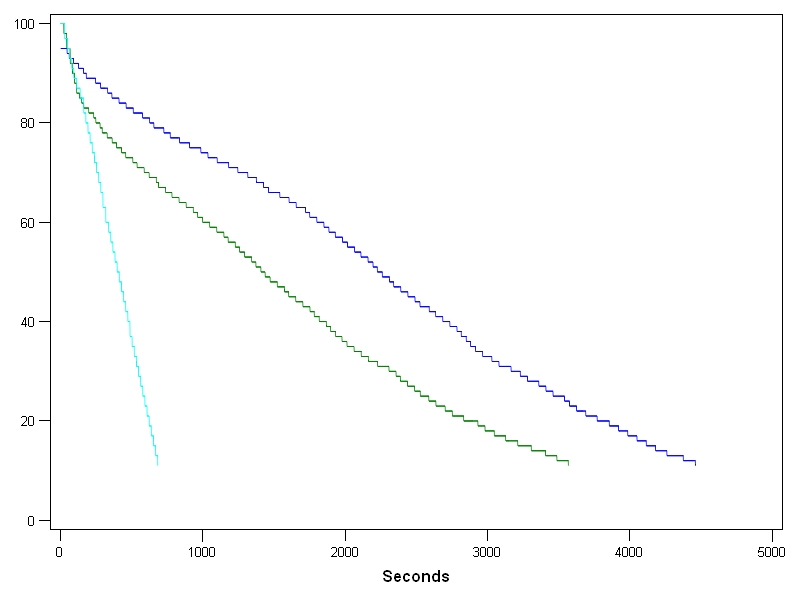
\includegraphics[width=7in]{battery.jpg} 
   \caption{Three Battery Profiles}
   \label{fig:battery}
\end{figure}
The line with the steepest slope corresponds to a run when the laptop was being subjected to a processor intensive process.  This caused the fan to run almost the entire time and the battery was depleted quickly.  The second steepest slope corresponds to a run when all Microsoft Office applications were open, but not used.  The least steep slope corresponds to a run where the laptop was in it's initial startup configuration with nothing but startup processes open.  

\section{Exiting SAS Processes at Power Threshold}
The hibernate or standby feature of most laptops is not always the
best method for ending a long running process in SAS.  If this is a
problem or if the system is operating on a UPS with limited off-AC
runtime it is nice to be able to cleanly exit the SAS process before
the system goes into hibernate or standby mode. This could easily be accomplished by periodically polling the battery status within a SAS program, and providing code to cleanly exit when the remaining percent falls below a pre-defined level.  For example, polling ended for the profile graphs generated above automatically when the battery percent remaining fell below 12\%.


\section{Conclusion}
Connecting SAS to the Windows API can be useful in many ways.  The
GetSystemPowerSource function allows SAS to query the battery a
laptop or UPS system.  This functionality can be used to build power
drain curves for various power configurations, or to control SAS
processes when the power level falls below a certain threshold.
\section{References}

\begin{tabular}[t]{llll}
\textbf{Required}
&   \SASregistered with the Windows API & David H. Johnson \\
& \multicolumn{2}{l}{\tiny\url{
http://www2.sas.com/proceedings/sugi30/248-30.pdf
}}\\
\textbf{Recommended} &   SASCBTBL Routine Statements & Richard A. DeVenezia \\
& \multicolumn{2}{l}{\tiny\url{
http://www.devenezia.com/downloads/sas/sascbtbl/
}}\\
&   GetSystemPowerStatus on MSDN & Microsoft Corporation \\
& \multicolumn{2}{l}{\tiny\url{
http://msdn.microsoft.com/library/default.asp?url=/library/en-us/power/base/getsystempowerstatus.asp
}}\\
\end{tabular}

\section{Acknowledgments}

Techniques from David Johnson and Richard DeVenezia's papers on using the Windows API within SAS make up the bulk of this paper  

\section{Contact Information}
Your comments and questions are valued and encouraged.

Contact the author(s):
%\begin{tabular}[c]{ll}%both columns are left justtified
\begin{tabular}[t]{rl}%note: double backslash(\\): newline
Name               & Samuel T. Croker                \\\
%Address            & 123 Main St                      \\
City, State, ZIP   & Lexington, SC 29073               \\
%Work Phone:        & 987-654-1234                     \\
%Fax:               & 987-654-3210                     \\
E-mail:            & scoyote@scoyote.net        \\
%Web:               & mycompany.com                    \\
\end{tabular}

\SASisRegisteredTrademark%macro variable provided by sugconf.cls
\OtherTrademarks%macro variable provided by sugconf.cls
\end{document}
